\chapter{HERO Architecture Simulation}
\label{chap:results}

To assess the performance of the HERO architecture a cycle accurate simulation
enviornment was implemented using SystemC and python. The enviornment was used
to a single configurations of the HERO architecture on real networks implemented
in pytorch from the TIMM library. The simulator also enables a study of the HERO
architecture by allowing different configurations of HERO to be passed in during
simulation. This study is left as part of future work. The simulator is composed
of two parts. 1) A python based frontend that can analyse the performance
results of any pytorch network on a configuration of HERO. 2) A SystemC based
backend for cycle accurate simulations of HERO running convolution/linear layers. In
this chapter we will first discuss the simulation enviornment and it's
components in \autoref{chap:hero:sim_platform}. The results from simulating all
695 networks from TIMM using a small HERO instance are given
\autoref{chap:hero:results}.

\section{Simulation Enviornment}
\label{chap:hero:sim_platform}

\subsection{Python Frontend}
\label{chap:hero:sim_platform:frontend}

The python frontend depicted in \autoref{fig:frontend}, expects a list of pytorch models and a dictionary defining the
configuration of a HERO instance as inputs. The configuration specifies the unroll factors
for F, C, the list of kernels sizes supported in direct mode, and the on-chip
storage dedicated for input and output feature map reuse, as well as the maximum
line size in any IFmap tensor.  The output of the
frontend is a pandas dataframe containing the results from the backend
simulation of the network(s) on the specified hero instance.  
After the frontend
recieves the list of pytorch models, CIGAR extracts the dimensions of all
supported layers (Conv2D and Linear). Afterwhich two layer transformation
operations are performed. The first converts convolution layers that are
unsupported directly into equivalent (1, 1) convolutions as described in
\autoref{chap:dda:dataflow_dse:indirect_mode}. Additionally, linear layers are
reinterpreted as (1, 1) convolutions based on the proof derived from
\autoref{chap:dda:dataflow_dse:indirect_mode:conv_gemm_equiv:proof}. 
The HERO arch. config being
evaluated is used to determine what layers are supported directly
After all layers have been converted to equivelent layers
that are supported by HERO, a layer decomposition step is performed to
decompose layers that have featuremaps that are two large to fit in the
HERO's on-chip memory. 
After all layer transformations are
performed, the layers are converted to test cases and a testcase deduplication
operation is used to limit the number of simulation runs required to simulate the network(s)
on HERO. 
After the testcase queue is generated it gets passed off to several
worker threads that manage independent backend instances that simulate the different
layers of the input network(s) concurrently. Note that since we're only
concerned with the architecutre metrics produced by the simulation the layers being
simulated don't use real weights and featuremaps from a forward inference pass
of the original network. Instead equivelent layer weights and featuremaps are
instantiated in the backend to avoid unnecessary transfer of data between the
front and backend.      


\begin{figure}[ht]
    \centering
    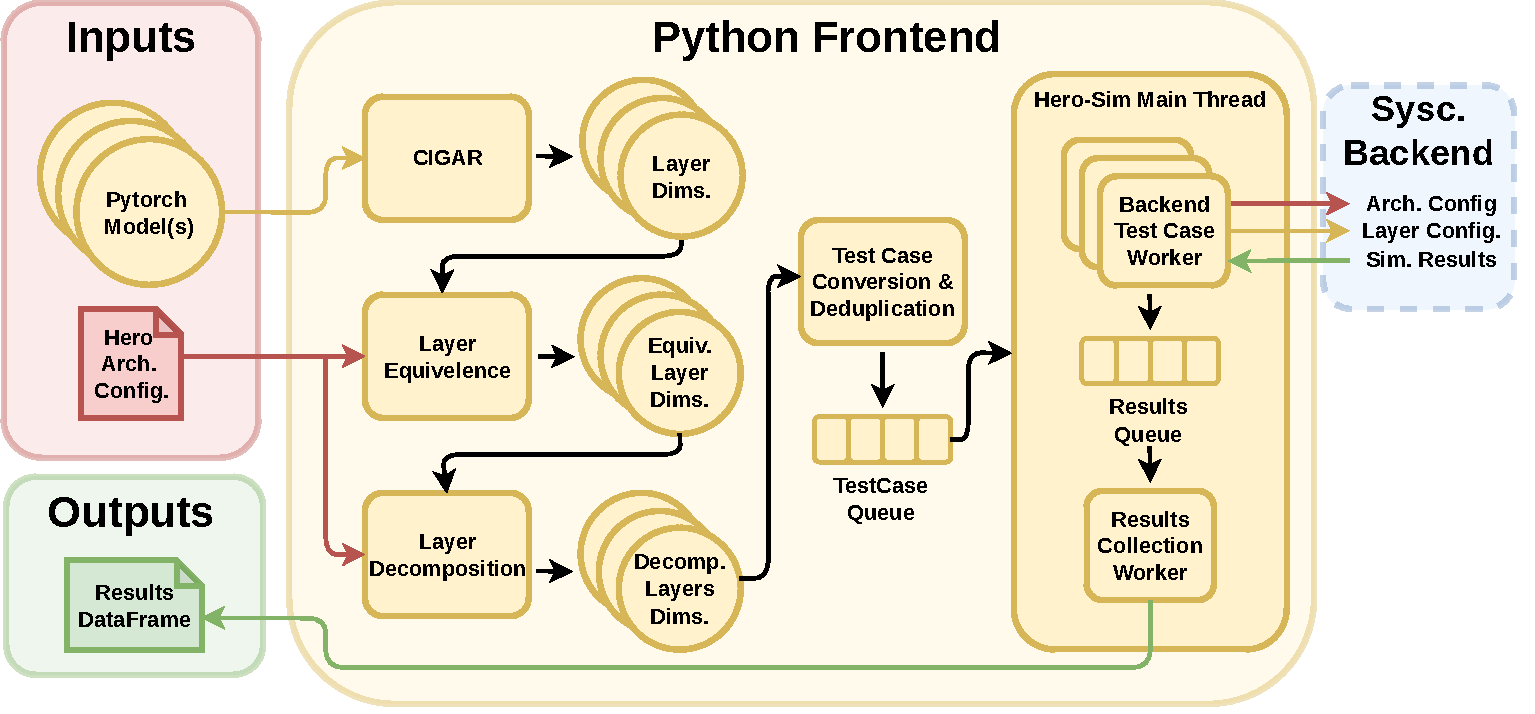
\includegraphics[scale=0.58]{fig/hero-sim-frontend.pdf}
    \caption{Illustration of the simulation enviornment's python frontend}
    \label{fig:frontend}
\end{figure}


\subsection{SystemC backend}
\label{chap:hero:sim_platform:backend}

The SystemC backend depicted in \autoref{fig:backend}, expects all inputs to be passed in as command line
arguments. The main inputs are 1) architecture configuration and 2) layer
configuration needed for simulation by the frontend. Sim results are generated
and sent back to the frontend using protobufs. The backend first instantiates a
HERO instance using the architecute configuration passed as input. Then it
generates an equivelent layer based on the input layer configuration. Finally
using both layer and architecture configuration it generates the SAM descriptors
required to perform all data movement operations on-chip. A dram load is then
simulated in zero time to transfer the layer data and descriptors to the on-chip
memories of the newly constructed HERO instance. Once the initialized HERO
instance is ready, the cycle accurate simulation starts and continues until all
SAMs reach a suspend descriptor. Then a dram load operation is again performed
in zero time to transfer the results from the HERO instance for validation.
After the simulated dram load, a protobuf is constructed, then populated with
the result of ouput validation and simulation results (assuming validation
success) and sent back to the frontend for further analysis and aggregation. 

The backend simulates interactions between the architecture and DRAM
functionally, in zero-time to avoid the complexity of DRAM and SAM interactions.
The interaction between SAMs and DRAM are left as part of future work. 

\begin{figure}[ht]
    \centering
    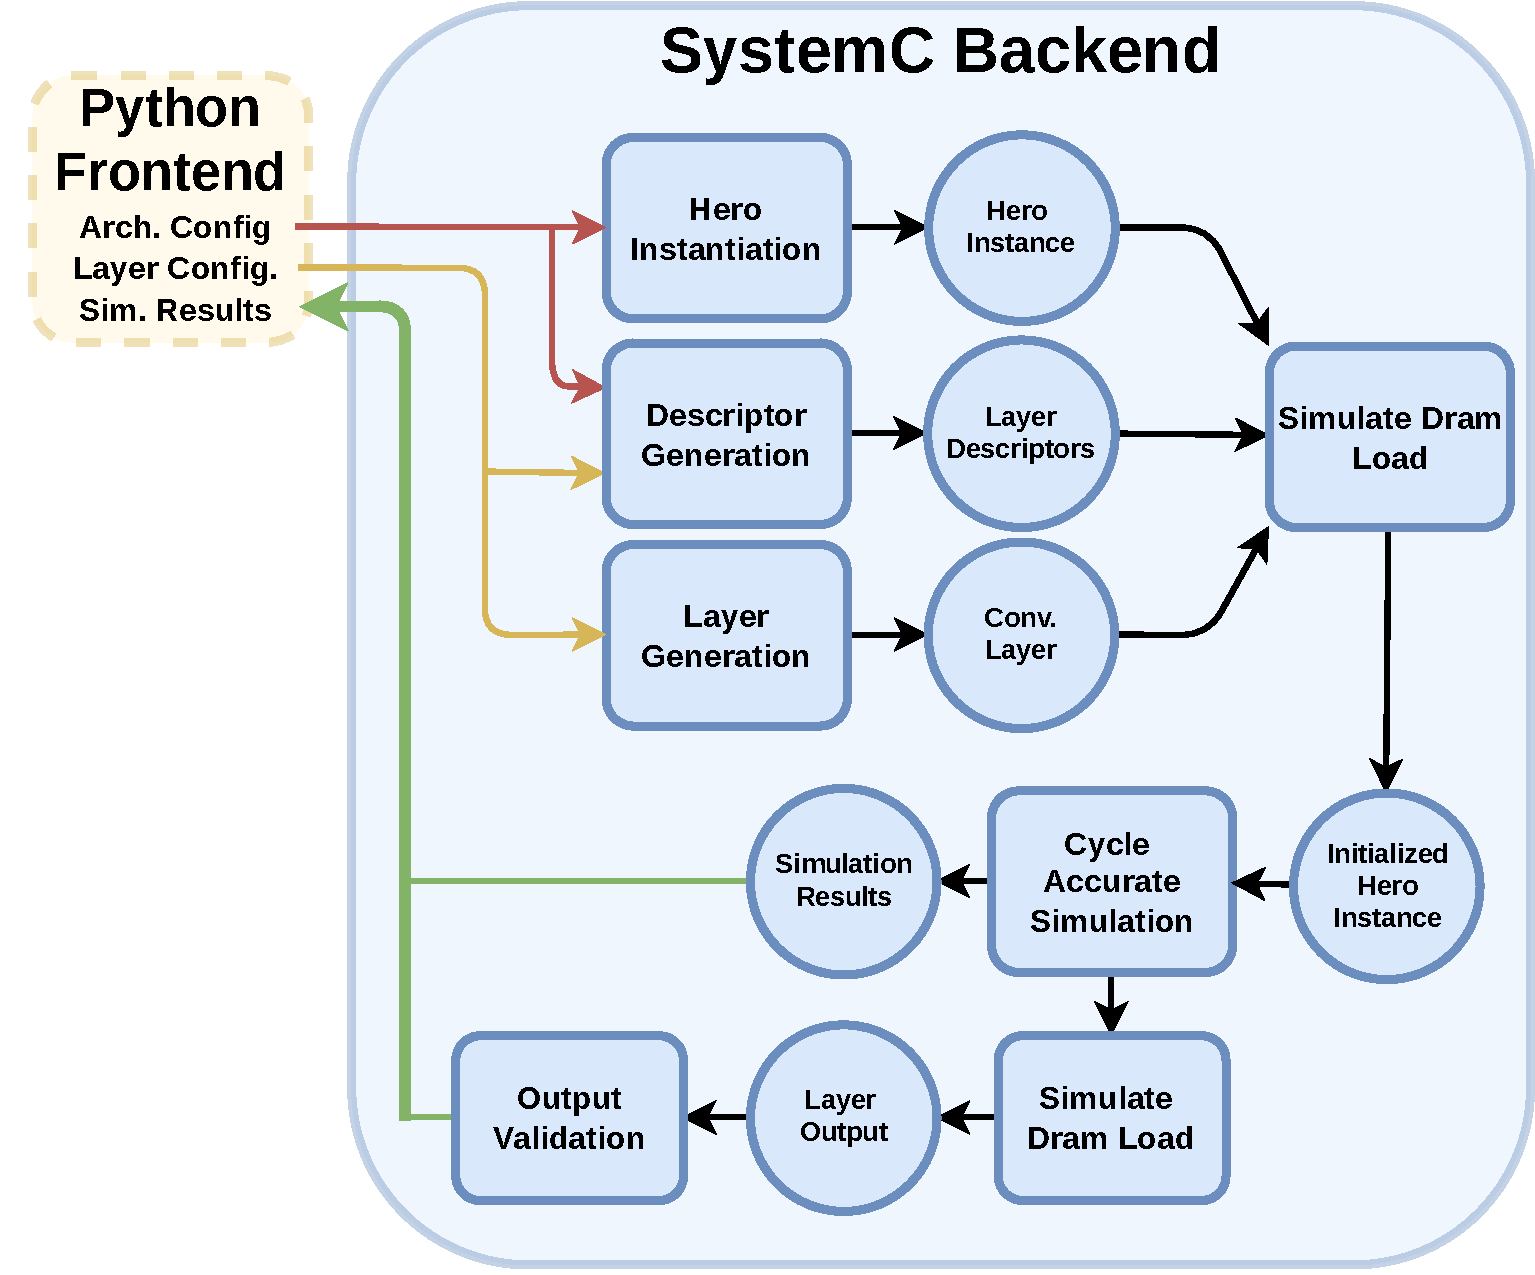
\includegraphics[scale=0.5]{fig/hero-sim-backend.pdf}
    \caption{Illustration of the simulation enviornment's SystemC backend}
    \label{fig:backend}
\end{figure}

\section{Experimental Results}
\label{chap:hero:results}

The configuration for the simulated architecture is given in
\autoref{tab:hero_config} based on the dimensions discovered in
\autoref{chap:dataflow_dse:exploring:results} and the sizing conclusions from
\autoref{chap:dataflow_dse:memory_hierarchy_sizing}. Note that sizes for on-chip
storage are given in the aggregate. The number of banks for IFmap L3 and OFmap
storage scales with the chosen $F_{unroll}$ and $C_{unroll}$ factors chosen. As
a result, the size of individual IFmap L3 and OFmap bank is proportional with
the overall size of IFmap L3 and OFmap on-chip storage but inversely
proportional with the chosen unroll factors. The CPU baseline used in this work
is an AMD 5950X processor. Thankfully since most networks in the TIMM library
have very similair layer configurations, the total number of both convolution
and linears layers to simulate on HERO are reduced from 182773 to 6048. As a
result, the total simulation time for all 695 Networks was around ~1.5 hours.
The layers simulated (convolution and linear) represent a substantial portion of
total network computation as show in \autoref{fig:percent_of_compute}. 

\begin{figure}[ht]
    \centering
    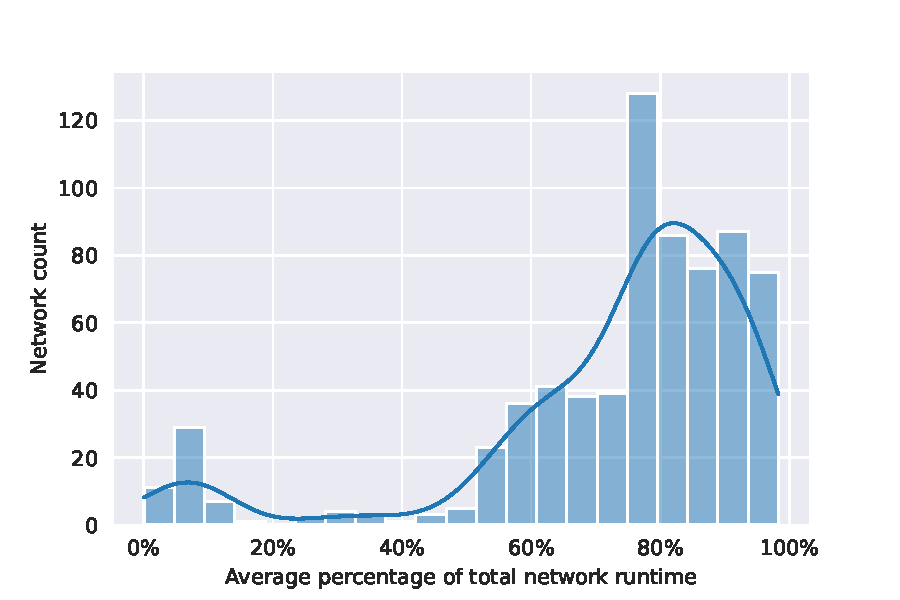
\includegraphics[scale=0.58]{Plots/overview/percent.pdf}
    \caption{Percent of computation represented by layers studied in the TIMM library}
    \label{fig:percent_of_compute}
\end{figure}

To determine percentage of compute Pytorch can be used to estimate the
total number of MAC operations used by natively supported layers. Unfortunately
many networks use custom layers constructed with pytorch primitives. For
each of these layers an analytical expression would need to be created to calculate
the number of operations in these layers. In the interest of time the runtimes
of these layers on a CPU were used to estimate computational demand. In
\autoref{fig:percent_of_compute}, the horizontal access defines the average
percentage of total network runtime taken up by supported layers. The vertical
axis defines the number of networks where convolution and linear layers take up
x\% of the computation where x is defined on the horizontal axis. From
\autoref{fig:percent_of_compute} it can be seen that the convolution and linear
layers represent the majority of network runtimes in the TIMM library. 

\begin{table}[]
    \center
    \begin{tabular}{|l|l|}
    \toprule
    Config. Param. & On-Chip Storage in Bytes    \\ 
    \midrule
    Weight Storage            & 16 B / PE (8 bit precision)  \\ \hline
    IFmap L3 Storage          & ~1 MB (8 bit precision)   \\ \hline
    IFmap L2 Storage          & 512 B (8 bit precision)   \\ \hline
    OFmap Storage             & 1 MB (16 bit precision)   \\ \hline
    $C_{unroll}$              & 18   \\ \hline
    $f_{unroll}$              & 32   \\ \hline
    Directly Supported Kernels             & {(1, 1), (3, 3)}   \\ \hline
    Assumed CLK Speed             & 1 Ghz   \\ \hline
\end{tabular}
\caption{HERO configuration used for analysis}
\label{tab:hero_config}
\end{table}

\subsection{Utilization}
\label{chap:hero:results:utilization}

Utilization can be used as a surrogate for how well layers map to the selected
HERO architecture based on the dataflow optimizations discussed in
\autoref{chap:arch_dimensioning}. From figure
\autoref{fig:network_layer_level_utilization} we can see that some networks benefit substantially from the architecture while
others don't. Network level distribution of average layer utilization is generally flat with
about a third of networks not benefiting from the architecture due to low
utilization. Low utilization is defined as average PE utilization throughout a
layer's computation that's less than 50\%.  


\begin{figure}
    \centering
    \subfigure[]{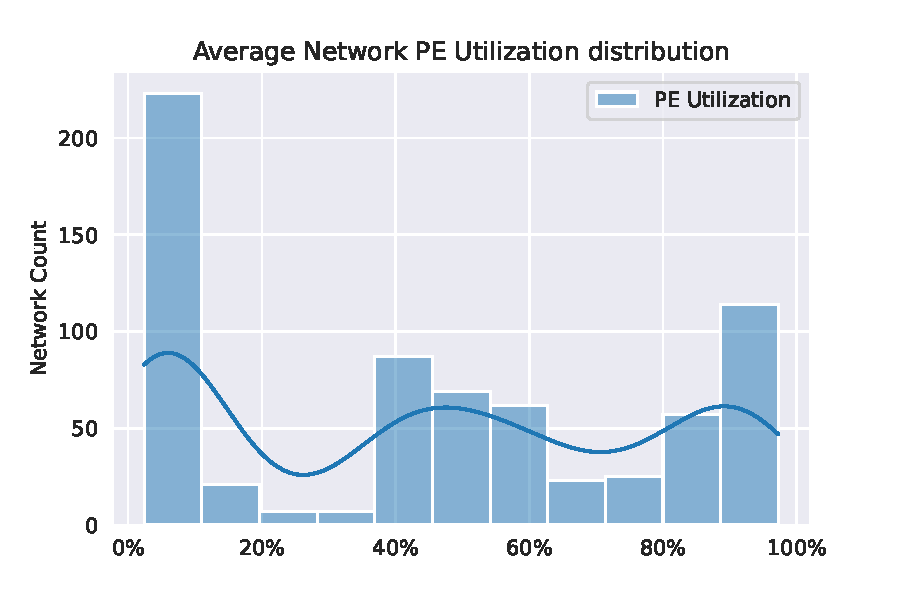
\includegraphics[width=0.48\textwidth]{Plots/utilization/network.pdf}}
    \hspace{0.1cm} 
    \subfigure[]{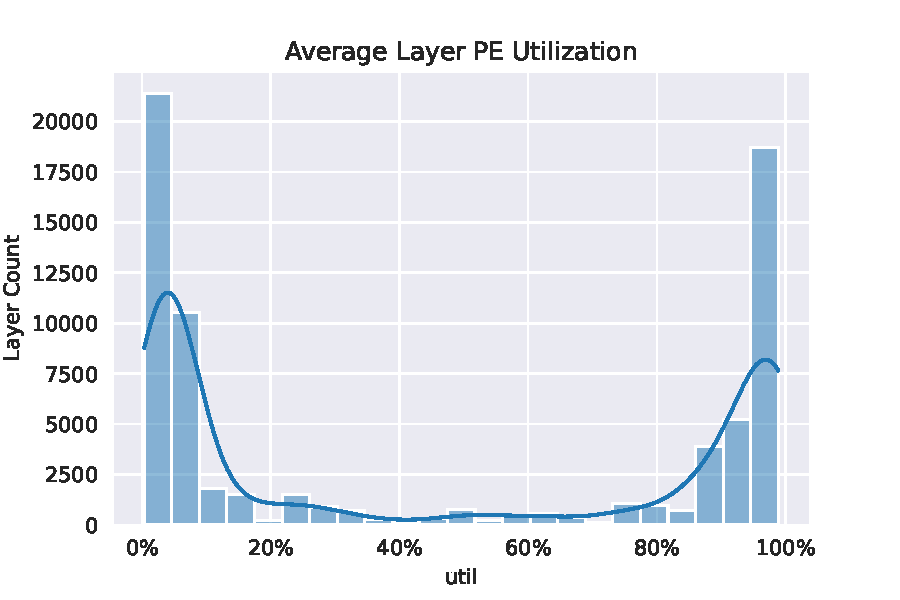
\includegraphics[width=0.48\textwidth]{Plots/utilization/layers.pdf}}
    \caption{Average layer utilization distributions by a) Network, b)Layer}
    \label{fig:network_layer_level_utilization}
\end{figure}

At the layer level we can see a more pronounced disparity in how much the
architecture benefits some layers over others. The next series of figures will
explore the cause of this disparity in utilization. If the cause of low
utilization in most layers is layer size as defined by number of operations then
utilization would generally scale with number of operations. Figure
\autoref{fig:utilization_macs_scaling} shows that the expected trend of
utilization scaling with MACS generally holds. However for a portion of the
layers on the bottom right utilization is low while MACs ops are high. This low
utilization would be especially concerning if combined with a speedup factor
$<1X$ over CPU baseline for that layer. One possible cause of low utilization,
combined with high MAC OPs and low speedup could be a high layer memory
footprint. To examine the effect of layer memory footprint as a cause for low
utilization, a scatter plot of layer feature map size vs utilization is
presented in \autoref{fig:scatter_plot_util_vs_fmap}. 


\begin{figure}[ht]
    \centering
    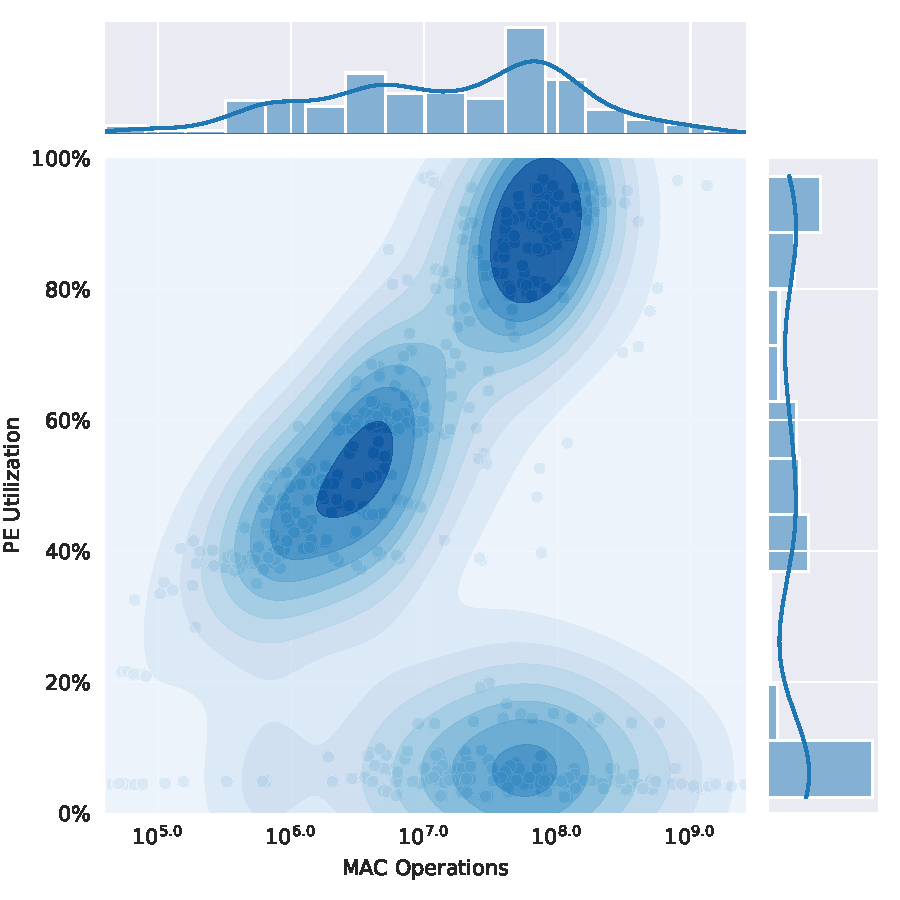
\includegraphics[scale=0.58]{Plots/utilization/util_vs_macs.pdf}
    \caption{Shaded contour plot of average layer utilization vs number of MACs}
    \label{fig:utilization_macs_scaling}
\end{figure}

Maybe layer decomposition and on chip memory plays a role here
Scatter plot of layers with speedup < 1 

From \autoref{fig:scatter_plot_util_vs_fmap} memory footprint doesn't matter no
clear trend 

For layers with low utilization

Layer type is a better predictor

Depthwise/Grouped map poorly to the architecture

Some non depthwise map poorly? Why?

They don't have enough channels and filters, PEs are under utilized
Individual channels and filters can be large though

Like depthwise, other types of concurrency need to be exploited

\begin{figure}
    \centering
    \subfigure[]{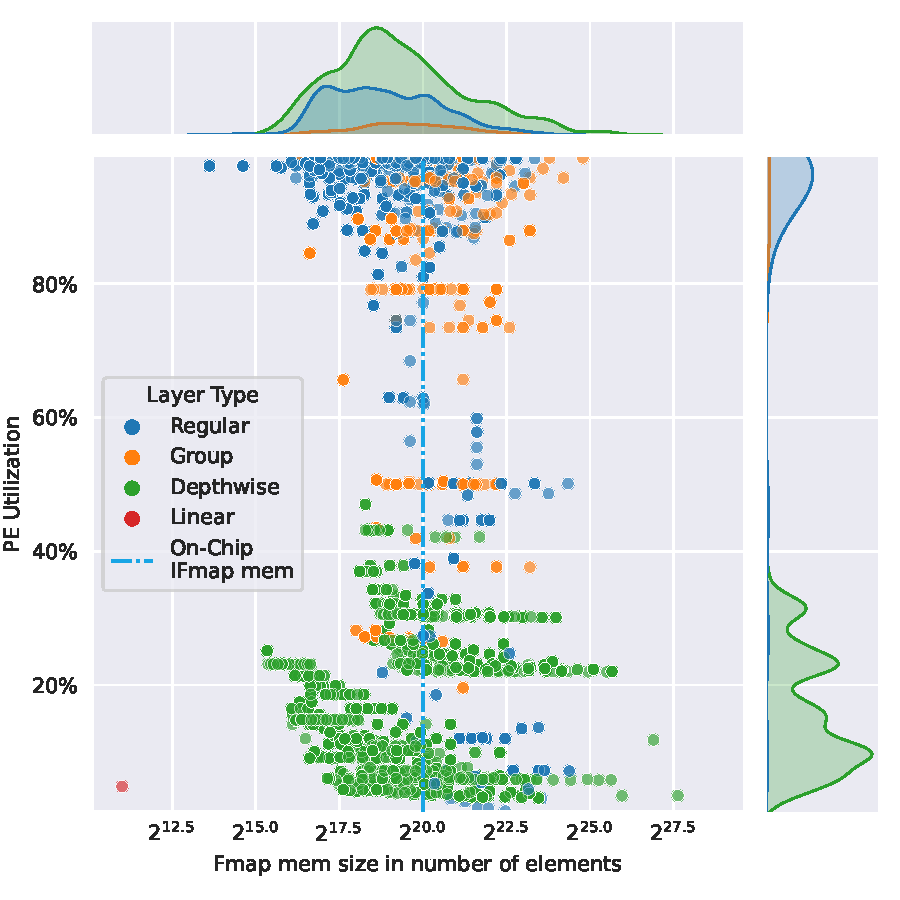
\includegraphics[width=0.48\textwidth]{Plots/utilization/util_vs_ifmap.pdf}}
    \hspace{0.1cm} 
    \subfigure[]{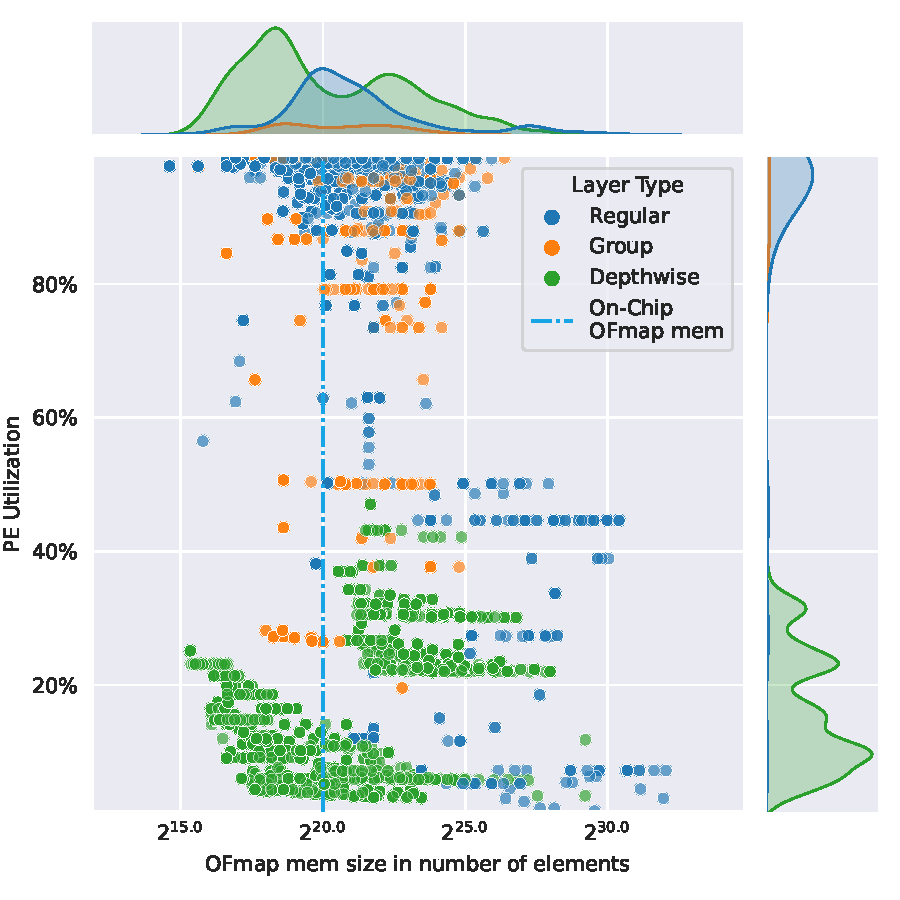
\includegraphics[width=0.48\textwidth]{Plots/utilization/util_vs_ofmap.pdf}}
    \caption{Average layer utilization distributions by a) Network, b)Layer}
    \label{fig:scatter_plot_util_vs_fmap}
\end{figure}

\begin{figure}
    \centering
    \subfigure[]{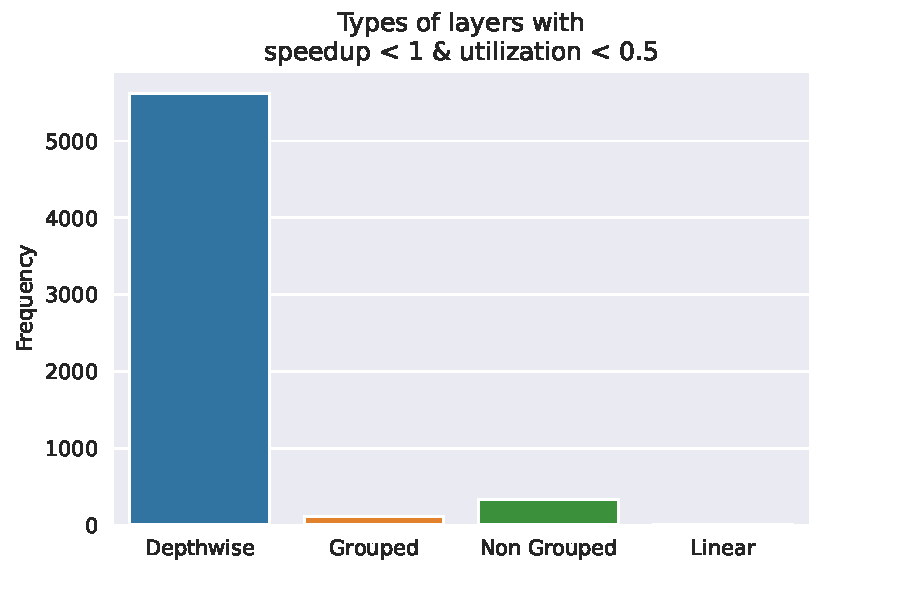
\includegraphics[width=0.48\textwidth]{Plots/utilization/type_of_low_util.pdf}}
    \hspace{0.1cm} 
    \subfigure[]{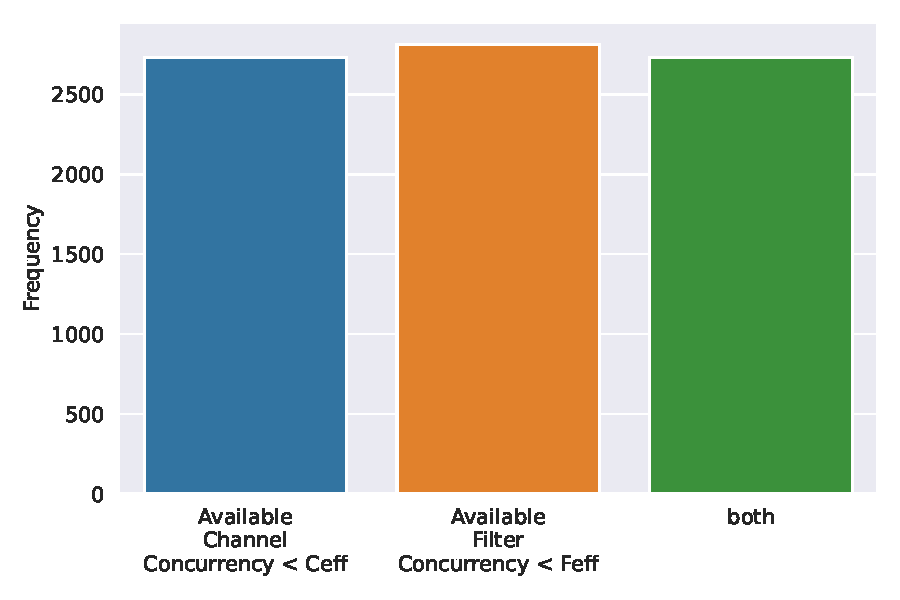
\includegraphics[width=0.48\textwidth]{Plots/utilization/low_util_big_fmap.pdf}}
    \caption{Average layer utilization distributions by a) Network, b)Layer}
    \label{fig:scatter_plot_util_vs_fmap}
\end{figure}

Some layers have high util, but low speedup
Those layers generally have really high C/F vs Ceff vs Feff
So we don't have resources for these layers

For layers with high util, low speedup and sane C/Ceff and F/Feff ratios 
are all lowered/lifted this increases their MACs which makes CPU competitve
given it's allowance for more varied kernel sizes

\begin{figure}
    \centering
    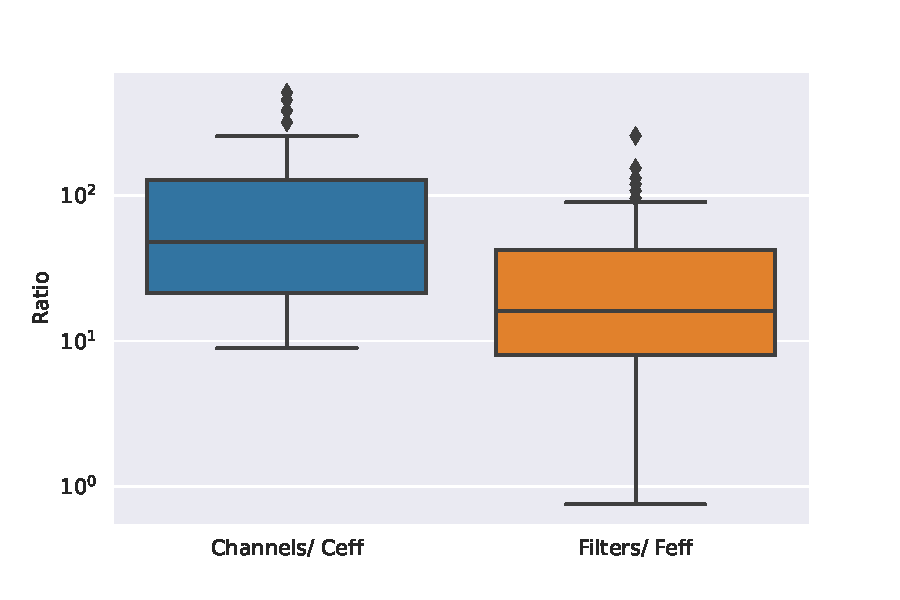
\includegraphics[scale=0.48]{Plots/utilization/ratios.pdf}
    \hspace{0.1cm} 
    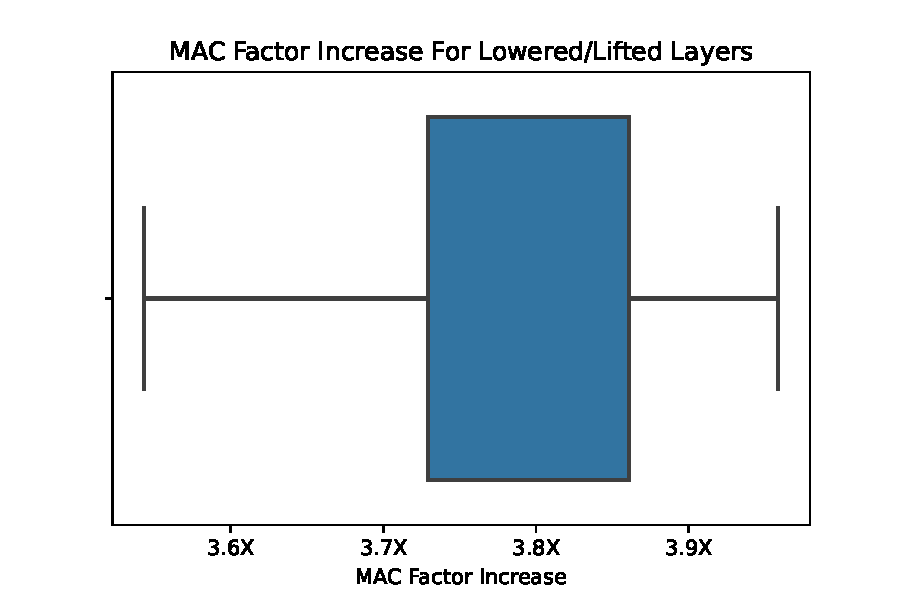
\includegraphics[scale=0.48]{Plots/utilization/macs.pdf}
    \caption{Average layer utilization distributions by a) Network, b)Layer}
    \label{fig:scatter_plot_util_vs_fmap}
\end{figure}

\subsection{Latency and Speedup over CPU Baseline}
\label{chap:hero:sim_platform:cigar_side}


most networks/ layers benefit
mean network speedup is over 

\begin{figure}[ht]
    \centering
    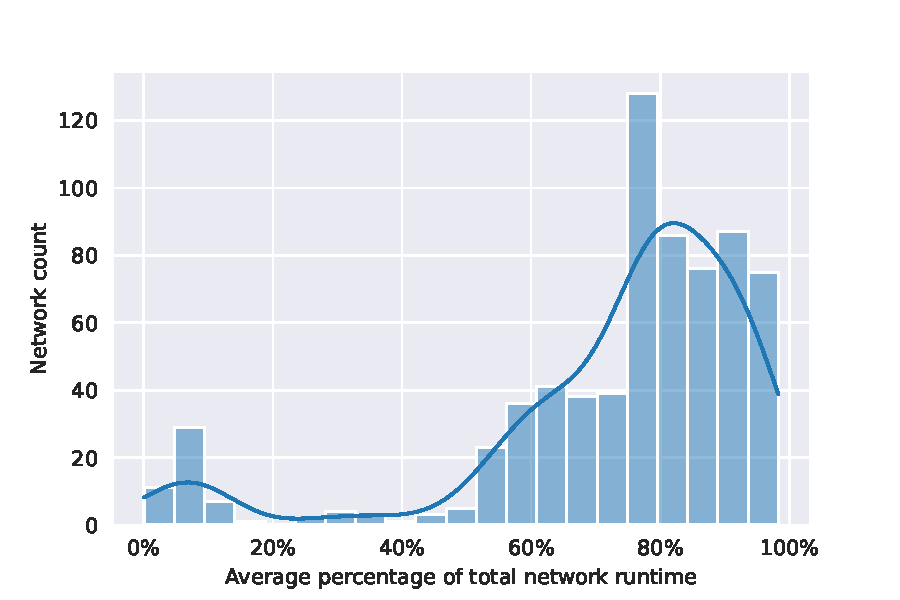
\includegraphics[scale=0.58]{Plots/overview/percent.pdf}
    \caption{Hardware Implementation Taxonomy adapted from \cite{maestro}}
    \label{fig:hw_taxonomy}
\end{figure}

Some networks don't benefit

\begin{figure}[ht]
    \centering
    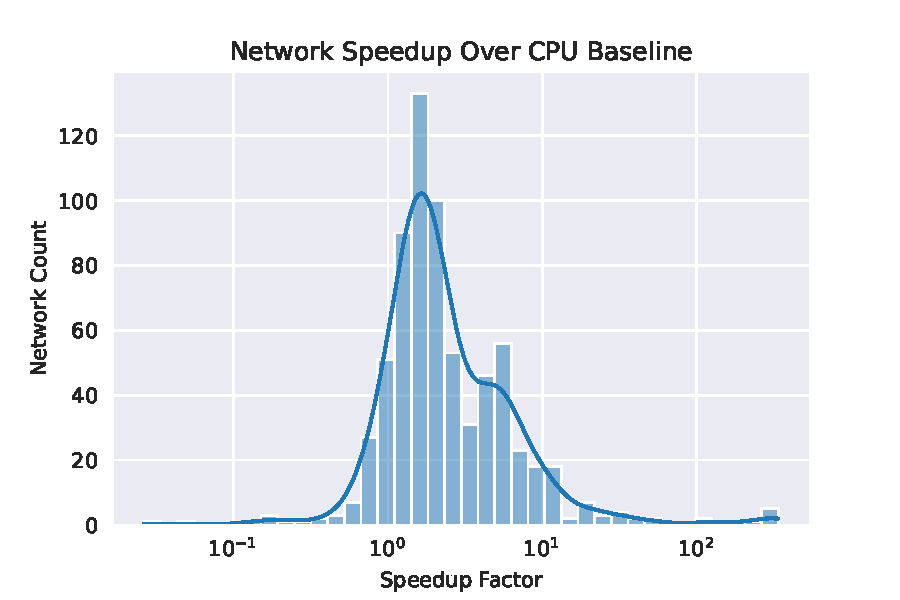
\includegraphics[scale=0.58]{Plots/latency/net_speedup.pdf}
    \caption{Hardware Implementation Taxonomy adapted from \cite{maestro}}
    \label{fig:hw_taxonomy}
\end{figure}

12\% of layers don't benefit

\begin{figure}[ht]
    \centering
    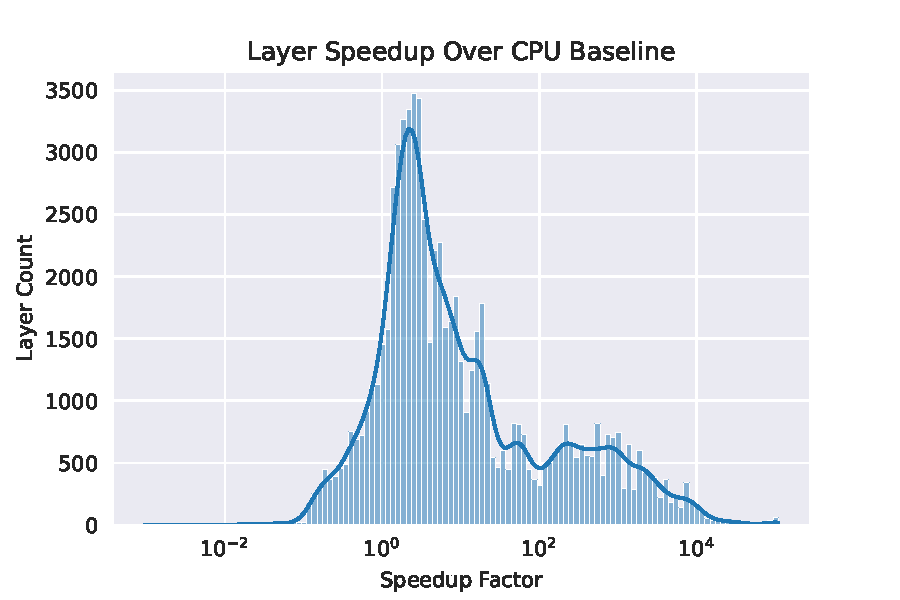
\includegraphics[scale=0.58]{Plots/latency/layer_speedup.pdf}
    \caption{Hardware Implementation Taxonomy adapted from \cite{maestro}}
    \label{fig:hw_taxonomy}
\end{figure}


why? see utilization
here's a boxplot of per layer speedup excluding layers with no speedup

\begin{figure}[ht]
    \centering
    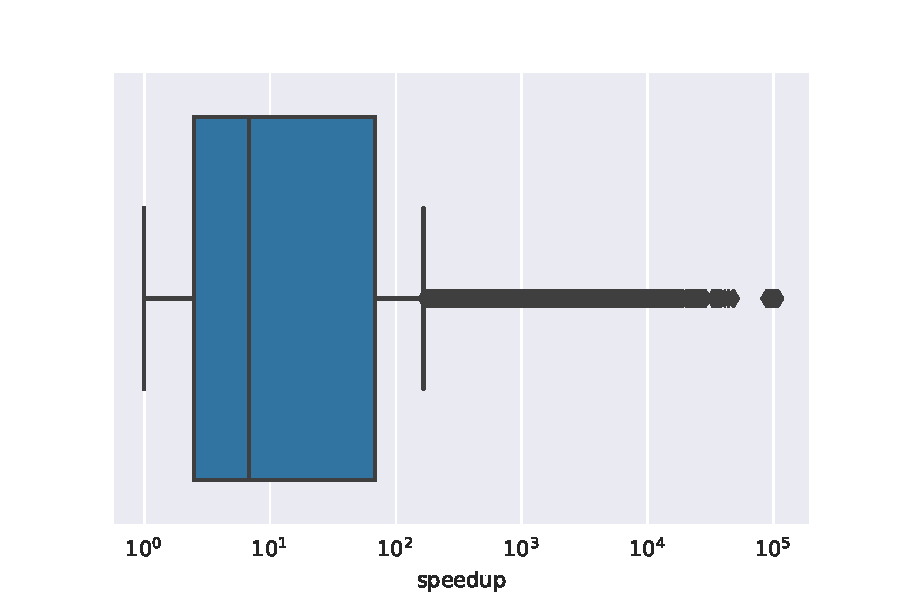
\includegraphics[scale=0.58]{Plots/latency/speedup_gt_1_boxplot.pdf}
    \caption{Hardware Implementation Taxonomy adapted from \cite{maestro}}
    \label{fig:hw_taxonomy}
\end{figure}

estimated fps based on supported layers, note that this should be taken as upper
bound because unsupported supported layers may take up more of the runtime than
anticipated (references earlier figure)

\begin{figure}[ht]
    \centering
    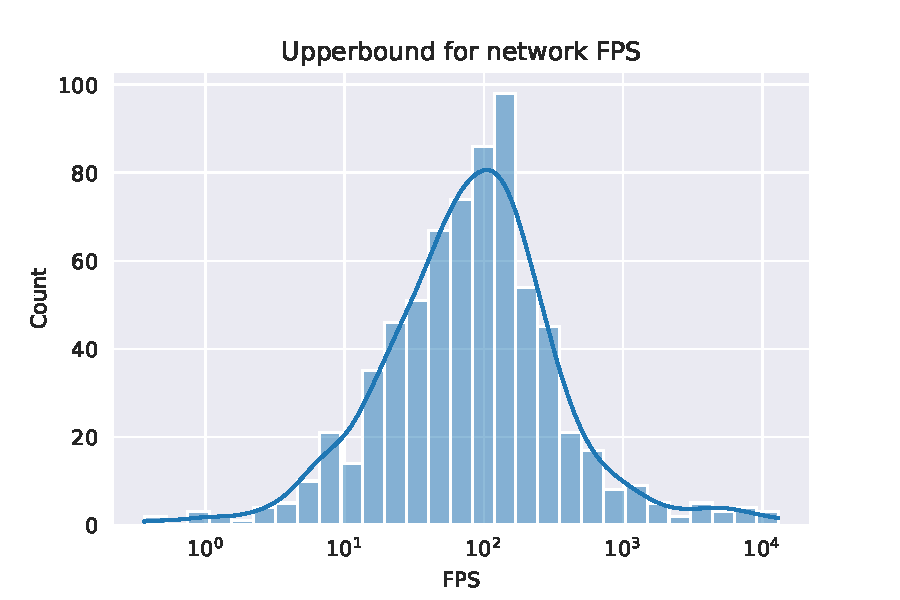
\includegraphics[scale=0.58]{Plots/latency/fps.pdf}
    \caption{Hardware Implementation Taxonomy adapted from \cite{maestro}}
    \label{fig:hw_taxonomy}
\end{figure}



\subsection{DRAM Bandwidth}
\label{chap:hero:sim_platform:cigar_side}

network and layer bandwidth histograms
within ddr4 spec? cite here

\begin{figure}[ht]
    \centering
    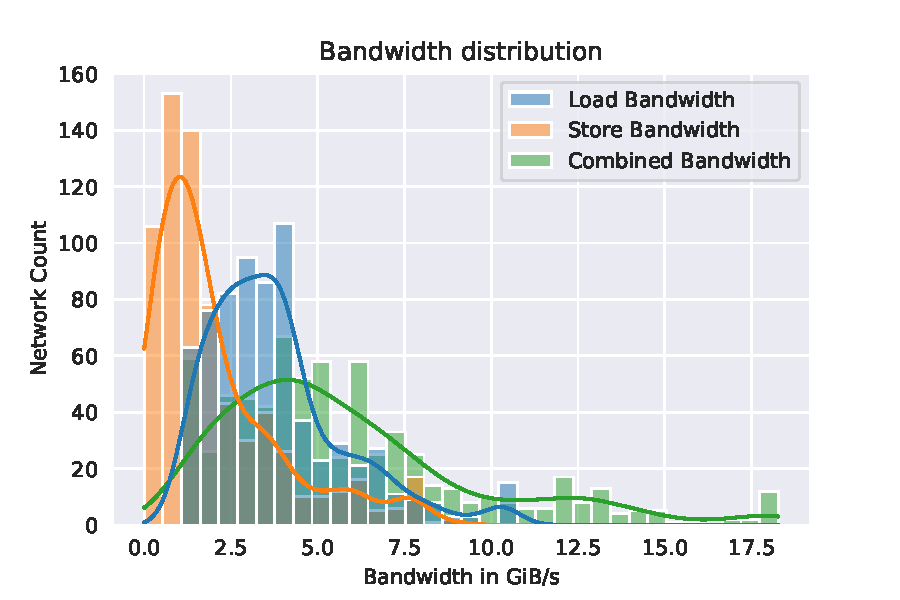
\includegraphics[scale=0.58]{Plots/resources/net_bw.pdf}
    \caption{Hardware Implementation Taxonomy adapted from \cite{maestro}}
    \label{fig:hw_taxonomy}
\end{figure}


\subsection{Energy}
\label{chap:hero:sim_platform:cigar_side}

used energy model in cite energy model
add energy model as table

\begin{figure}[ht]
    \centering
    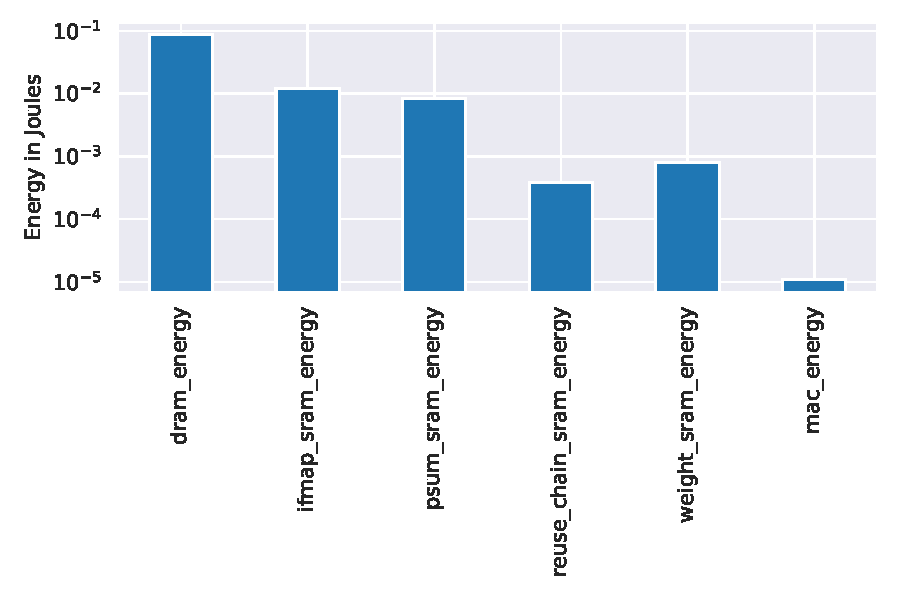
\includegraphics[scale=0.58]{Plots/energy/barplot.pdf}
    \caption{Hardware Implementation Taxonomy adapted from \cite{maestro}}
    \label{fig:hw_taxonomy}
\end{figure}

mac is basically free
dram dominates

network inferences/ j median is around 57

\begin{figure}[ht]
    \centering
    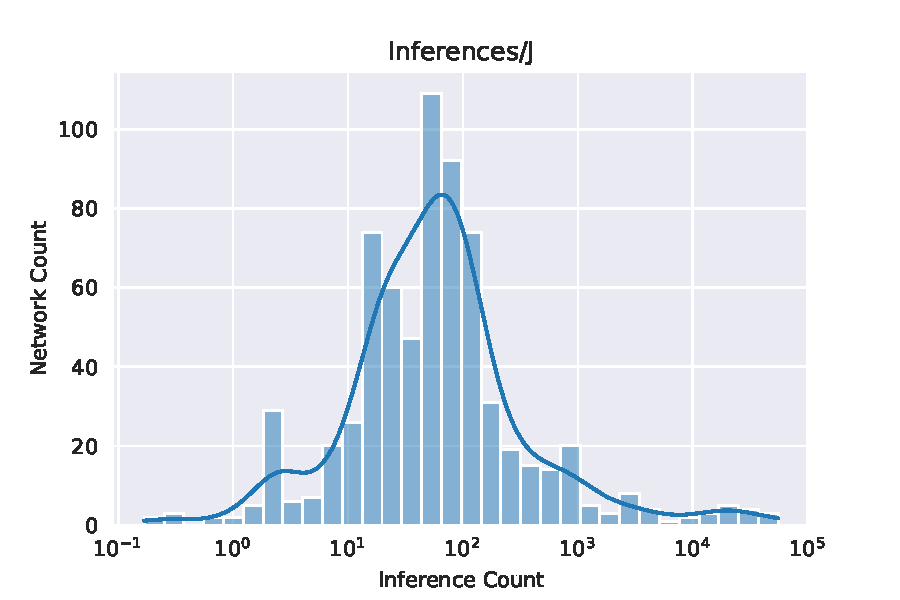
\includegraphics[scale=0.58]{Plots/energy/inferences.pdf}
    \caption{Hardware Implementation Taxonomy adapted from \cite{maestro}}
    \label{fig:hw_taxonomy}
\end{figure}


excluding dram number jumps to 20K
there's room to reduce on-chip data movement by exploiting different kinds of
concurrency

\begin{figure}[ht]
    \centering
    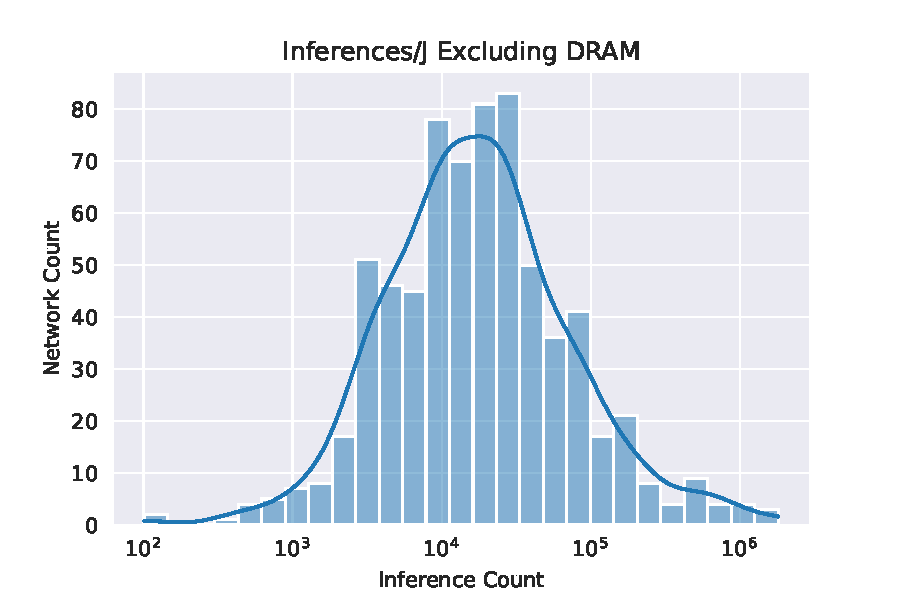
\includegraphics[scale=0.58]{Plots/energy/inferences_wo_dram.pdf}
    \caption{Hardware Implementation Taxonomy adapted from \cite{maestro}}
    \label{fig:hw_taxonomy}
\end{figure}

\subsection{Area}
\label{chap:conv_gemm_equiv:overhead}

area model as table
bulk goes to ofmap storage and ifmap storage
ofmap storage requires higher precision

\begin{figure}[ht]
    \centering
    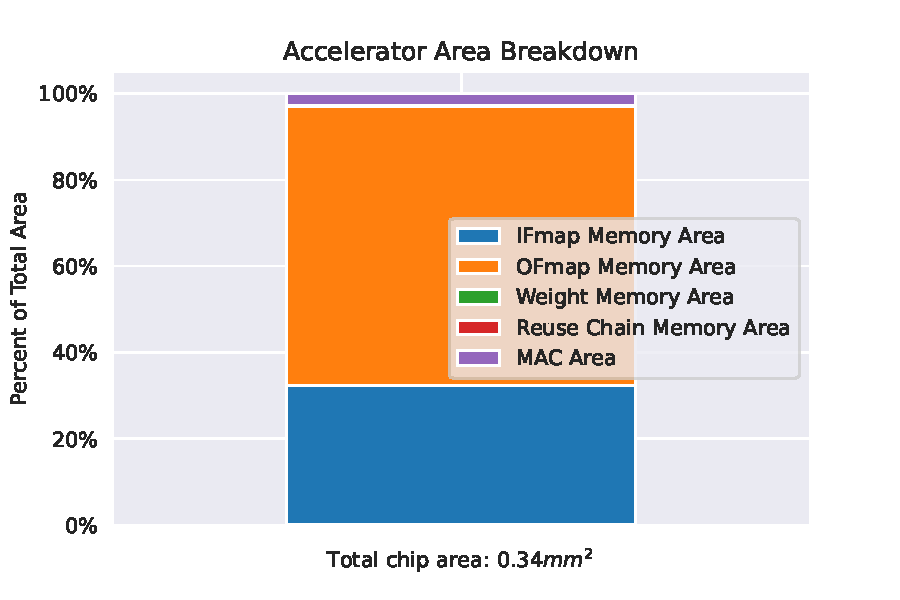
\includegraphics[scale=0.58]{Plots/resources/area.pdf}
    \caption{Hardware Implementation Taxonomy adapted from \cite{maestro}}
    \label{fig:hw_taxonomy}
\end{figure}

\subsection{Descriptor program scaling}
\label{chap:hero:sim_platform:cigar_side}

median required storage for descriptors per address generator is around 100
scaling can be improved with more complicated descriptors

\begin{figure}[ht]
    \centering
    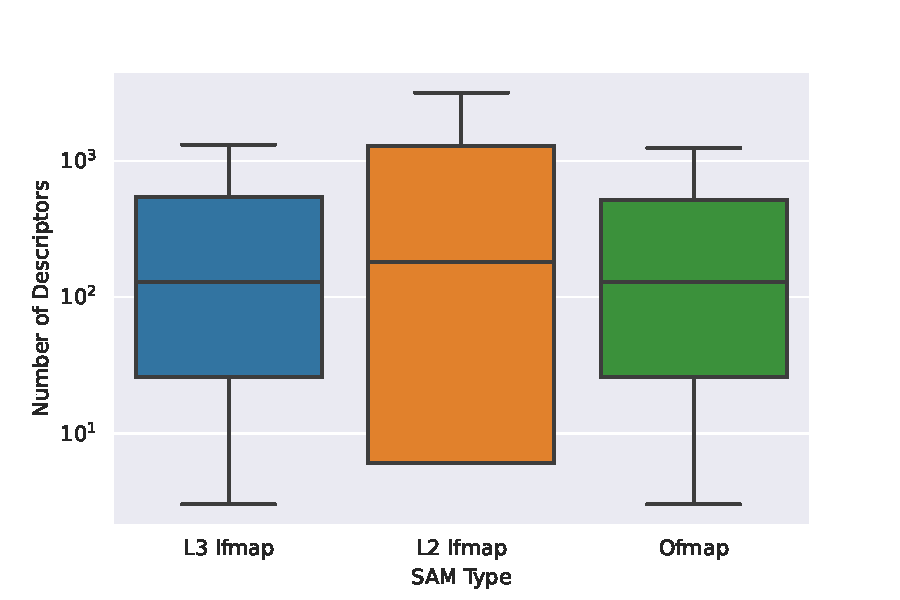
\includegraphics[scale=0.58]{Plots/resources/descriptors.pdf}
    \caption{Hardware Implementation Taxonomy adapted from \cite{maestro}}
    \label{fig:hw_taxonomy}
\end{figure}

\subsection{Per network results}
\label{chap:hero:sim_platform:cigar_side}

networks chosen
resnet50 (popular and backbone for alot of other networks)
mobilenetv3 specific to edge devices and has depthwise layers

\subsubsection{ResNet50}

\clearpage
\begin{center}
    \begin{tabular}{lrlrrlllll}
        \toprule
        {} &  Count & IFmap &     Cin &    Cout &       K &  Stride & Padding & Groups &   Bias \\
        Name     &        &             &         &         &         &         &         &        &        \\
        \midrule
        conv\_0   & 1 &  (224, 224) &     3.0 &    64.0 &  (7, 7) &  (2, 2) &  (3, 3) &    1.0 &  False \\
        conv\_1   & 1 &    (56, 56) &    64.0 &    64.0 &  (1, 1) &  (1, 1) &  (0, 0) &    1.0 &  False \\
        conv\_2   & 3 &    (56, 56) &    64.0 &    64.0 &  (3, 3) &  (1, 1) &  (1, 1) &    1.0 &  False \\
        conv\_3   & 4 &    (56, 56) &    64.0 &   256.0 &  (1, 1) &  (1, 1) &  (0, 0) &    1.0 &  False \\
        conv\_4   & 2 &    (56, 56) &   256.0 &    64.0 &  (1, 1) &  (1, 1) &  (0, 0) &    1.0 &  False \\
        conv\_5   & 1 &    (56, 56) &   256.0 &   128.0 &  (1, 1) &  (1, 1) &  (0, 0) &    1.0 &  False \\
        conv\_6   & 1 &    (56, 56) &   128.0 &   128.0 &  (3, 3) &  (2, 2) &  (1, 1) &    1.0 &  False \\
        conv\_7   & 4 &    (28, 28) &   128.0 &   512.0 &  (1, 1) &  (1, 1) &  (0, 0) &    1.0 &  False \\
        conv\_8   & 1 &    (56, 56) &   256.0 &   512.0 &  (1, 1) &  (2, 2) &  (0, 0) &    1.0 &  False \\
        conv\_9   & 3 &    (28, 28) &   512.0 &   128.0 &  (1, 1) &  (1, 1) &  (0, 0) &    1.0 &  False \\
        conv\_10  & 3 &    (28, 28) &   128.0 &   128.0 &  (3, 3) &  (1, 1) &  (1, 1) &    1.0 &  False \\
        conv\_11  & 1 &    (28, 28) &   512.0 &   256.0 &  (1, 1) &  (1, 1) &  (0, 0) &    1.0 &  False \\
        conv\_12  & 1 &    (28, 28) &   256.0 &   256.0 &  (3, 3) &  (2, 2) &  (1, 1) &    1.0 &  False \\
        conv\_13  & 6 &    (14, 14) &   256.0 &  1024.0 &  (1, 1) &  (1, 1) &  (0, 0) &    1.0 &  False \\
        conv\_14  & 1 &    (28, 28) &   512.0 &  1024.0 &  (1, 1) &  (2, 2) &  (0, 0) &    1.0 &  False \\
        conv\_15  & 5 &    (14, 14) &  1024.0 &   256.0 &  (1, 1) &  (1, 1) &  (0, 0) &    1.0 &  False \\
        conv\_16  & 5 &    (14, 14) &   256.0 &   256.0 &  (3, 3) &  (1, 1) &  (1, 1) &    1.0 &  False \\
        conv\_17  & 1 &    (14, 14) &  1024.0 &   512.0 &  (1, 1) &  (1, 1) &  (0, 0) &    1.0 &  False \\
        conv\_18  & 1 &    (14, 14) &   512.0 &   512.0 &  (3, 3) &  (2, 2) &  (1, 1) &    1.0 &  False \\
        conv\_19  & 3 &      (7, 7) &   512.0 &  2048.0 &  (1, 1) &  (1, 1) &  (0, 0) &    1.0 &  False \\
        conv\_20  & 1 &    (14, 14) &  1024.0 &  2048.0 &  (1, 1) &  (2, 2) &  (0, 0) &    1.0 &  False \\
        conv\_21  & 2 &      (7, 7) &  2048.0 &   512.0 &  (1, 1) &  (1, 1) &  (0, 0) &    1.0 &  False \\
        conv\_22  & 2 &      (7, 7) &   512.0 &   512.0 &  (3, 3) &  (1, 1) &  (1, 1) &    1.0 &  False \\
        linear\_0 & 1 &      (1, 1) &  2048.0 &  1000.0 &     N/A &     N/A &     N/A &    N/A &   True \\
        \bottomrule
        \end{tabular}
\end{center}

\subsubsection{MobilenetV3}
\begin{figure}[ht]
    \centering
    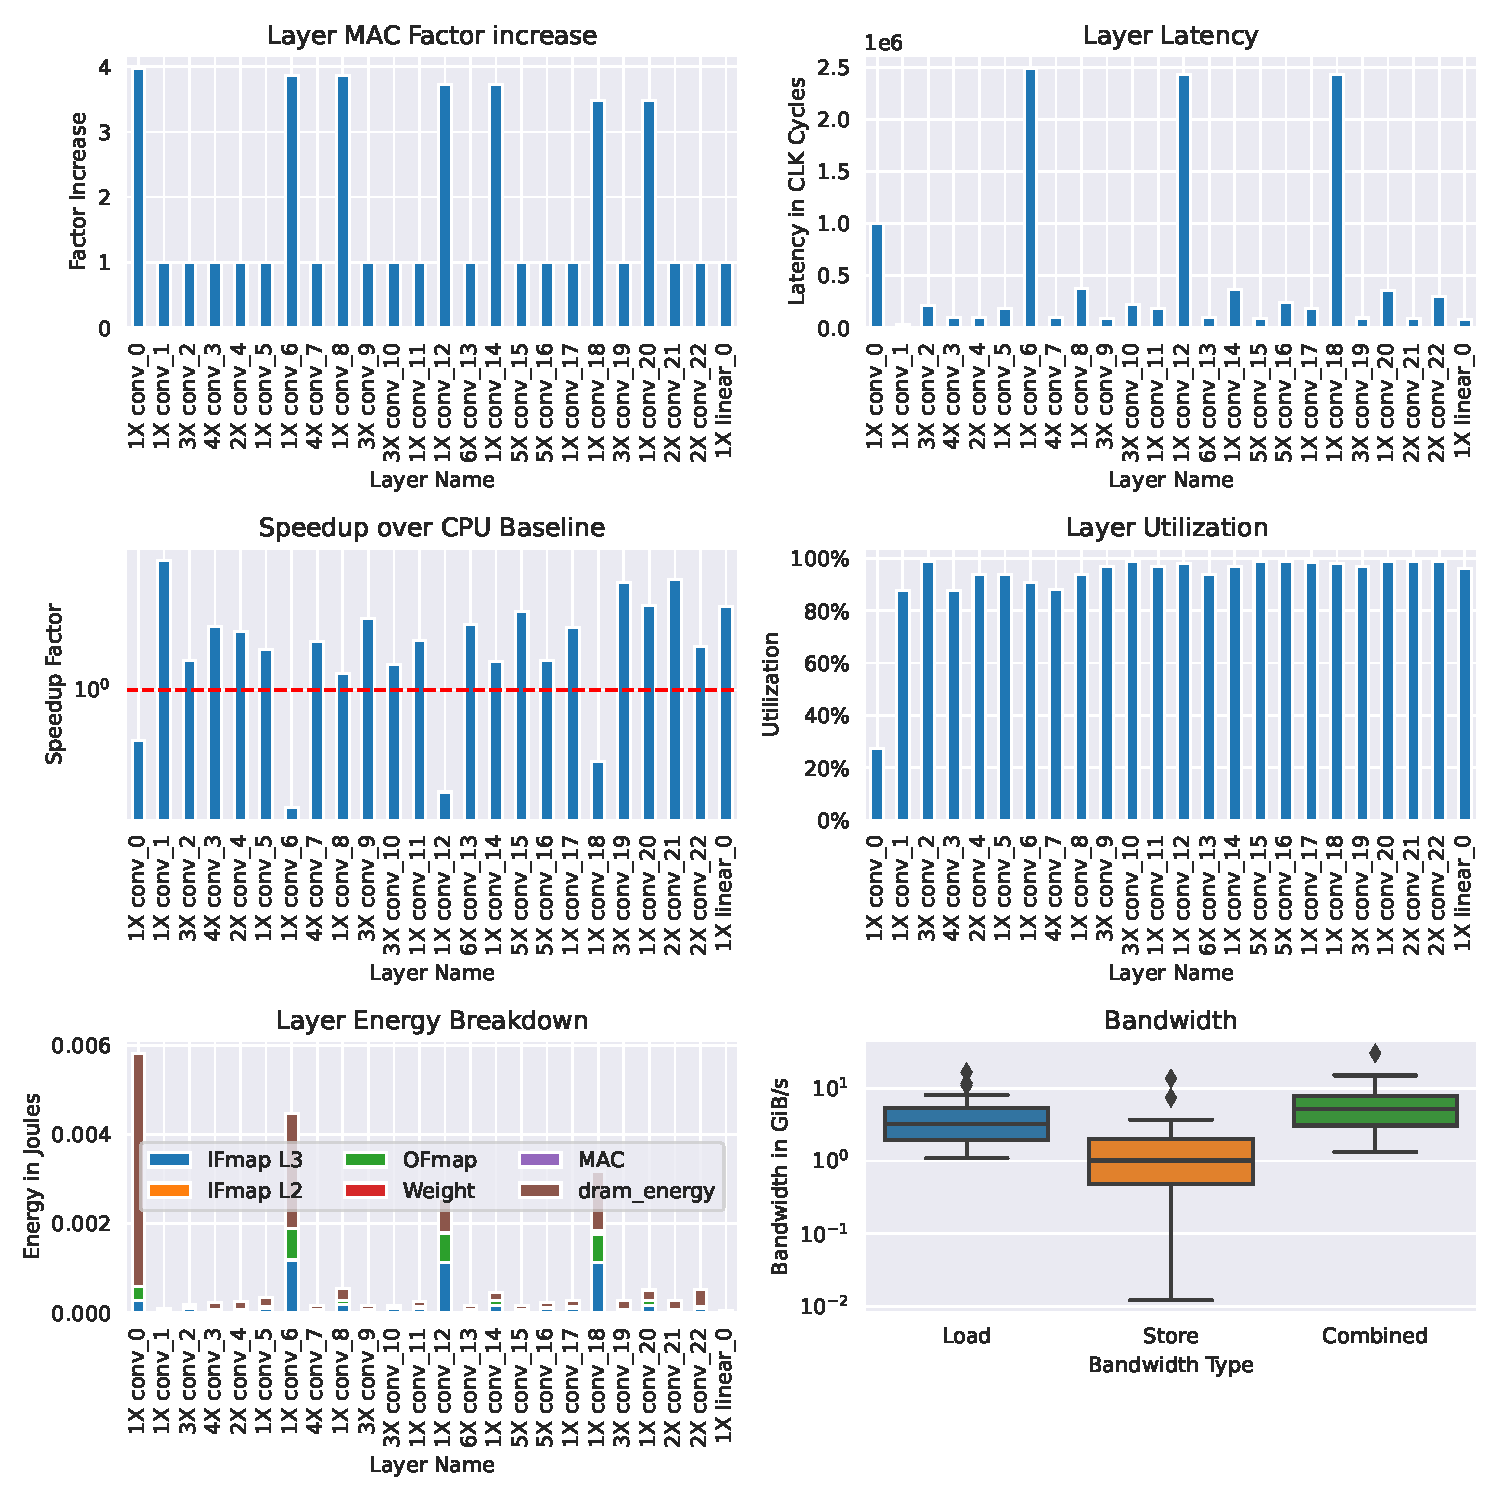
\includegraphics[scale=0.6]{Plots/networks/resnet50.pdf}
    \caption{Hardware Implementation Taxonomy adapted from \cite{maestro}}
    \label{fig:hw_taxonomy}
\end{figure}

\clearpage
% \Rotatebox{90}{%
\begin{center}
    \begin{tabular}{lrlrrlllll}
        \toprule
        {} &  Count &       IFmap &    Cin &    Cout &       K &  Stride & Padding & Groups &   Bias \\
        Name    &        &             &        &         &         &         &         &        &        \\
        \midrule
        conv\_0  &      1 &  (224, 224) &    3.0 &    16.0 &  (3, 3) &  (2, 2) &  (1, 1) &    1.0 &  False \\
        conv\_1  &      1 &  (112, 112) &   16.0 &    16.0 &  (3, 3) &  (2, 2) &  (1, 1) &   16.0 &  False \\
        conv\_2  &      1 &      (1, 1) &   16.0 &     8.0 &  (1, 1) &  (1, 1) &  (0, 0) &    1.0 &   True \\
        conv\_3  &      1 &      (1, 1) &    8.0 &    16.0 &  (1, 1) &  (1, 1) &  (0, 0) &    1.0 &   True \\
        conv\_4  &      1 &    (56, 56) &   16.0 &    16.0 &  (1, 1) &  (1, 1) &  (0, 0) &    1.0 &  False \\
        conv\_5  &      1 &    (56, 56) &   16.0 &    72.0 &  (1, 1) &  (1, 1) &  (0, 0) &    1.0 &  False \\
        conv\_6  &      1 &    (56, 56) &   72.0 &    72.0 &  (3, 3) &  (2, 2) &  (1, 1) &   72.0 &  False \\
        conv\_7  &      1 &    (28, 28) &   72.0 &    24.0 &  (1, 1) &  (1, 1) &  (0, 0) &    1.0 &  False \\
        conv\_8  &      1 &    (28, 28) &   24.0 &    88.0 &  (1, 1) &  (1, 1) &  (0, 0) &    1.0 &  False \\
        conv\_9  &      1 &    (28, 28) &   88.0 &    88.0 &  (3, 3) &  (1, 1) &  (1, 1) &   88.0 &  False \\
        conv\_10 &      1 &    (28, 28) &   88.0 &    24.0 &  (1, 1) &  (1, 1) &  (0, 0) &    1.0 &  False \\
        conv\_11 &      1 &    (28, 28) &   24.0 &    96.0 &  (1, 1) &  (1, 1) &  (0, 0) &    1.0 &  False \\
        conv\_12 &      1 &    (28, 28) &   96.0 &    96.0 &  (5, 5) &  (2, 2) &  (2, 2) &   96.0 &  False \\
        conv\_13 &      2 &      (1, 1) &   96.0 &    24.0 &  (1, 1) &  (1, 1) &  (0, 0) &    1.0 &   True \\
        conv\_14 &      2 &      (1, 1) &   24.0 &    96.0 &  (1, 1) &  (1, 1) &  (0, 0) &    1.0 &   True \\
        conv\_15 &      1 &    (14, 14) &   96.0 &    32.0 &  (1, 1) &  (1, 1) &  (0, 0) &    1.0 &  False \\
        conv\_16 &      2 &    (14, 14) &   32.0 &   192.0 &  (1, 1) &  (1, 1) &  (0, 0) &    1.0 &  False \\
        conv\_17 &      2 &    (14, 14) &  192.0 &   192.0 &  (5, 5) &  (1, 1) &  (2, 2) &  192.0 &  False \\
        conv\_18 &      2 &      (1, 1) &  192.0 &    48.0 &  (1, 1) &  (1, 1) &  (0, 0) &    1.0 &   True \\
        conv\_19 &      2 &      (1, 1) &   48.0 &   192.0 &  (1, 1) &  (1, 1) &  (0, 0) &    1.0 &   True \\
        conv\_20 &      2 &    (14, 14) &  192.0 &    32.0 &  (1, 1) &  (1, 1) &  (0, 0) &    1.0 &  False \\
        conv\_21 &      1 &    (14, 14) &   32.0 &    96.0 &  (1, 1) &  (1, 1) &  (0, 0) &    1.0 &  False \\
        conv\_22 &      1 &    (14, 14) &   96.0 &    96.0 &  (5, 5) &  (1, 1) &  (2, 2) &   96.0 &  False \\
        conv\_23 &      1 &    (14, 14) &   96.0 &    40.0 &  (1, 1) &  (1, 1) &  (0, 0) &    1.0 &  False \\
        conv\_24 &      1 &    (14, 14) &   40.0 &   120.0 &  (1, 1) &  (1, 1) &  (0, 0) &    1.0 &  False \\
        conv\_25 &      1 &    (14, 14) &  120.0 &   120.0 &  (5, 5) &  (1, 1) &  (2, 2) &  120.0 &  False \\
        conv\_26 &      1 &      (1, 1) &  120.0 &    32.0 &  (1, 1) &  (1, 1) &  (0, 0) &    1.0 &   True \\
        conv\_27 &      1 &      (1, 1) &   32.0 &   120.0 &  (1, 1) &  (1, 1) &  (0, 0) &    1.0 &   True \\
        conv\_28 &      1 &    (14, 14) &  120.0 &    40.0 &  (1, 1) &  (1, 1) &  (0, 0) &    1.0 &  False \\
        conv\_29 &      1 &    (14, 14) &   40.0 &   240.0 &  (1, 1) &  (1, 1) &  (0, 0) &    1.0 &  False \\
        conv\_30 &      1 &    (14, 14) &  240.0 &   240.0 &  (5, 5) &  (2, 2) &  (2, 2) &  240.0 &  False \\
        conv\_31 &      1 &      (1, 1) &  240.0 &    64.0 &  (1, 1) &  (1, 1) &  (0, 0) &    1.0 &   True \\
        conv\_32 &      1 &      (1, 1) &   64.0 &   240.0 &  (1, 1) &  (1, 1) &  (0, 0) &    1.0 &   True \\
        conv\_33 &      1 &      (7, 7) &  240.0 &    72.0 &  (1, 1) &  (1, 1) &  (0, 0) &    1.0 &  False \\
        conv\_34 &      3 &      (7, 7) &   72.0 &   432.0 &  (1, 1) &  (1, 1) &  (0, 0) &    1.0 &  False \\
        conv\_35 &      2 &      (7, 7) &  432.0 &   432.0 &  (5, 5) &  (1, 1) &  (2, 2) &  432.0 &  False \\
        conv\_36 &      2 &      (1, 1) &  432.0 &   112.0 &  (1, 1) &  (1, 1) &  (0, 0) &    1.0 &   True \\
        conv\_37 &      2 &      (1, 1) &  112.0 &   432.0 &  (1, 1) &  (1, 1) &  (0, 0) &    1.0 &   True \\
        conv\_38 &      2 &      (7, 7) &  432.0 &    72.0 &  (1, 1) &  (1, 1) &  (0, 0) &    1.0 &  False \\
        conv\_39 &      1 &      (1, 1) &  432.0 &  1024.0 &  (1, 1) &  (1, 1) &  (0, 0) &    1.0 &   True \\
        \bottomrule
        \end{tabular}
\end{center}


\begin{figure}[ht]
    \centering
    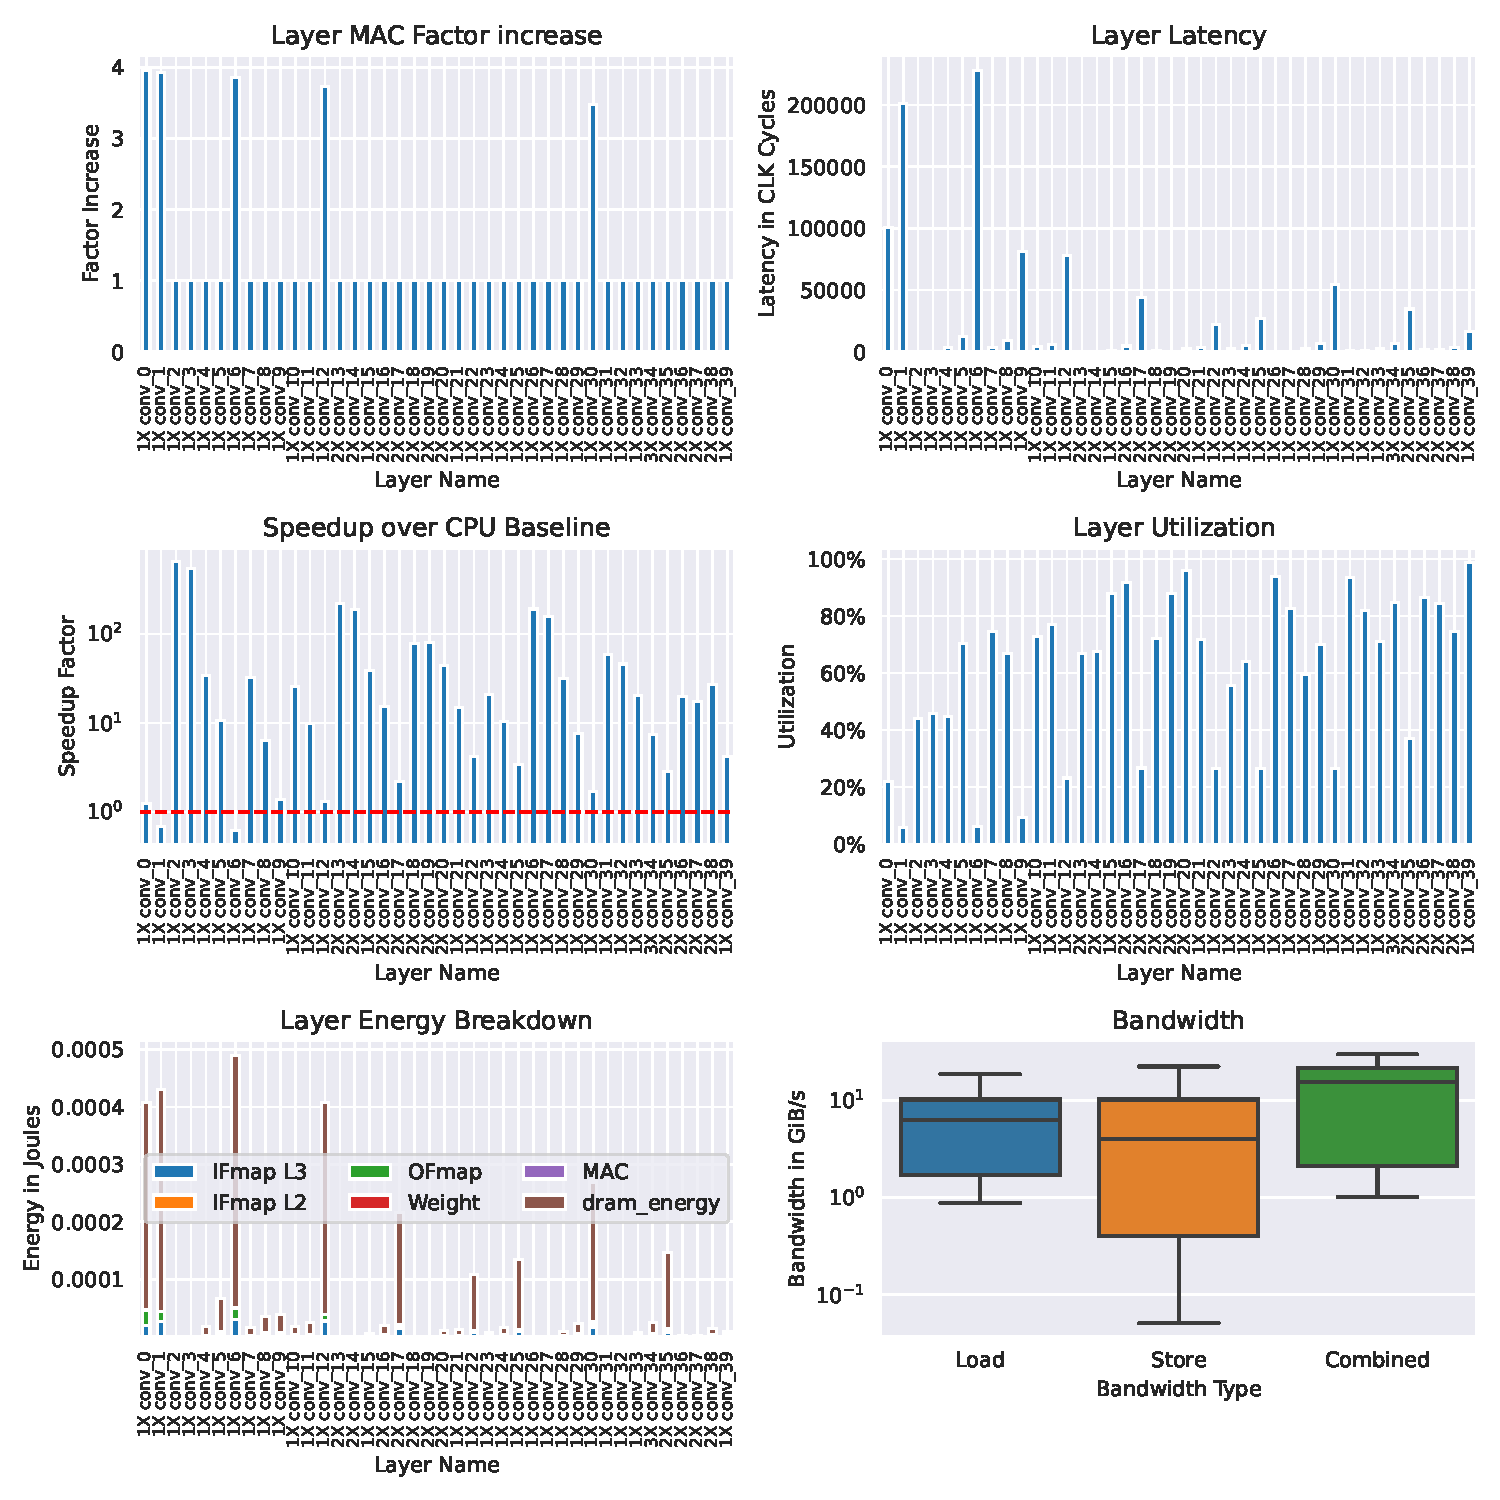
\includegraphics[scale=0.6]{Plots/networks/mobilenetv3_small_075.pdf}
    \caption{Hardware Implementation Taxonomy adapted from \cite{maestro}}
    \label{fig:hw_taxonomy}
\end{figure}
